编译器的目的是将源文件“翻译”成目标机器的汇编文件。为了减小在翻译过程中所面对的源语言和目标汇编语言之间的复杂程度差距,编译器一般会将源文件变换成若干种中间表示,这些中间表示同目标汇编语言的相似程度逐渐增大。同时,在一些中间表示上,编译器能够相对容易地进行语义检查;在另一些些中间表示上,编译器还能利用相对简单、与源语言和目标汇编语言分别隔离的中间表示来进行机器无关优化。

MiniC采用了两重中间表示:抽象语法树(Abstract Syntax Tree)和三元式。语义检查在前者上完成,机器无关优化在后者上完成。下面将介绍这两种中间表示的生成以及在其上所做的相关工作。

\section{抽象语法树AST}
\label{AST}
AST是MiniC采用的第一重中间表示,它由在词法/语法分析阶段生成。由于我们在AST上完成了符号表的生成和类型检查,因此这两部分也在本章介绍。
\subsection{生成}
\label{genAST}
AST的结构是根据上下文无关文法的产生式定义的:一个终结符节点是一棵AST;一棵以产生式左部非终结符为根的AST的子节点按从左到右顺序分别是其右部分法符号所产生的AST。

比如有如下产生式:
\begin{displaymath}
	A:=aBcD
\end{displaymath}
其中大写字母代表非终结符,小写字母代表终结符,那么以非终结符A为根的AST就是如下形式:
\dirtree{%
.1 A.
.2 a.
.2 以非终结符B为根的AST.
.2 c.
.2 以非终结符D为根的AST.
}
注意到AST的定义实际上也给出了其产生方法:只要在做LR分析时,随着规约的进行,将子树与根进行连接即可。

在实现时,AST的叶节点在词法分析时生成,内部节点在语法分析时在不同的产生式的语法规则指导下生成,并在规约时连接到其父节点上。

下面给出一个MiniC的AST节点所包含的内容:
\label{ASTnode}
\begin{lstlisting}
typedef struct AST_NODE{
  	int nodeType;//节点类型,即节点代表了哪个文法符号
  	int nodeLevel;//节点深度
	union node_content content; //节点包含的内容,只有叶子节点才不为空,在词法分析时添加
  	AST_NODE * father;//父节点
  	AST_NODE * leftChild;//最左子节点
  	AST_NODE * rightSibling;//右兄弟节点

	struct symtbl_hdr* symtbl;//文法符号所在范围的符号表
	AST_NODE* double_list;
}AST_NODE;
\end{lstlisting}
{\it \anchor 有关节点类型的详细定义,请参阅:\verb|AST.h|}\\
{\it \anchor 有关建立AST树的相应过程,请参阅:\verb|AST_operation.c|, \verb|minic.y|}\\
\subsection{生成的语法树示例}
我们利用\verb|dot|生成了下面代码的AST:
\begin{lstlisting}
int main()
{
	int i;
	i = i + 1;
}

\end{lstlisting}

\begin{center}
	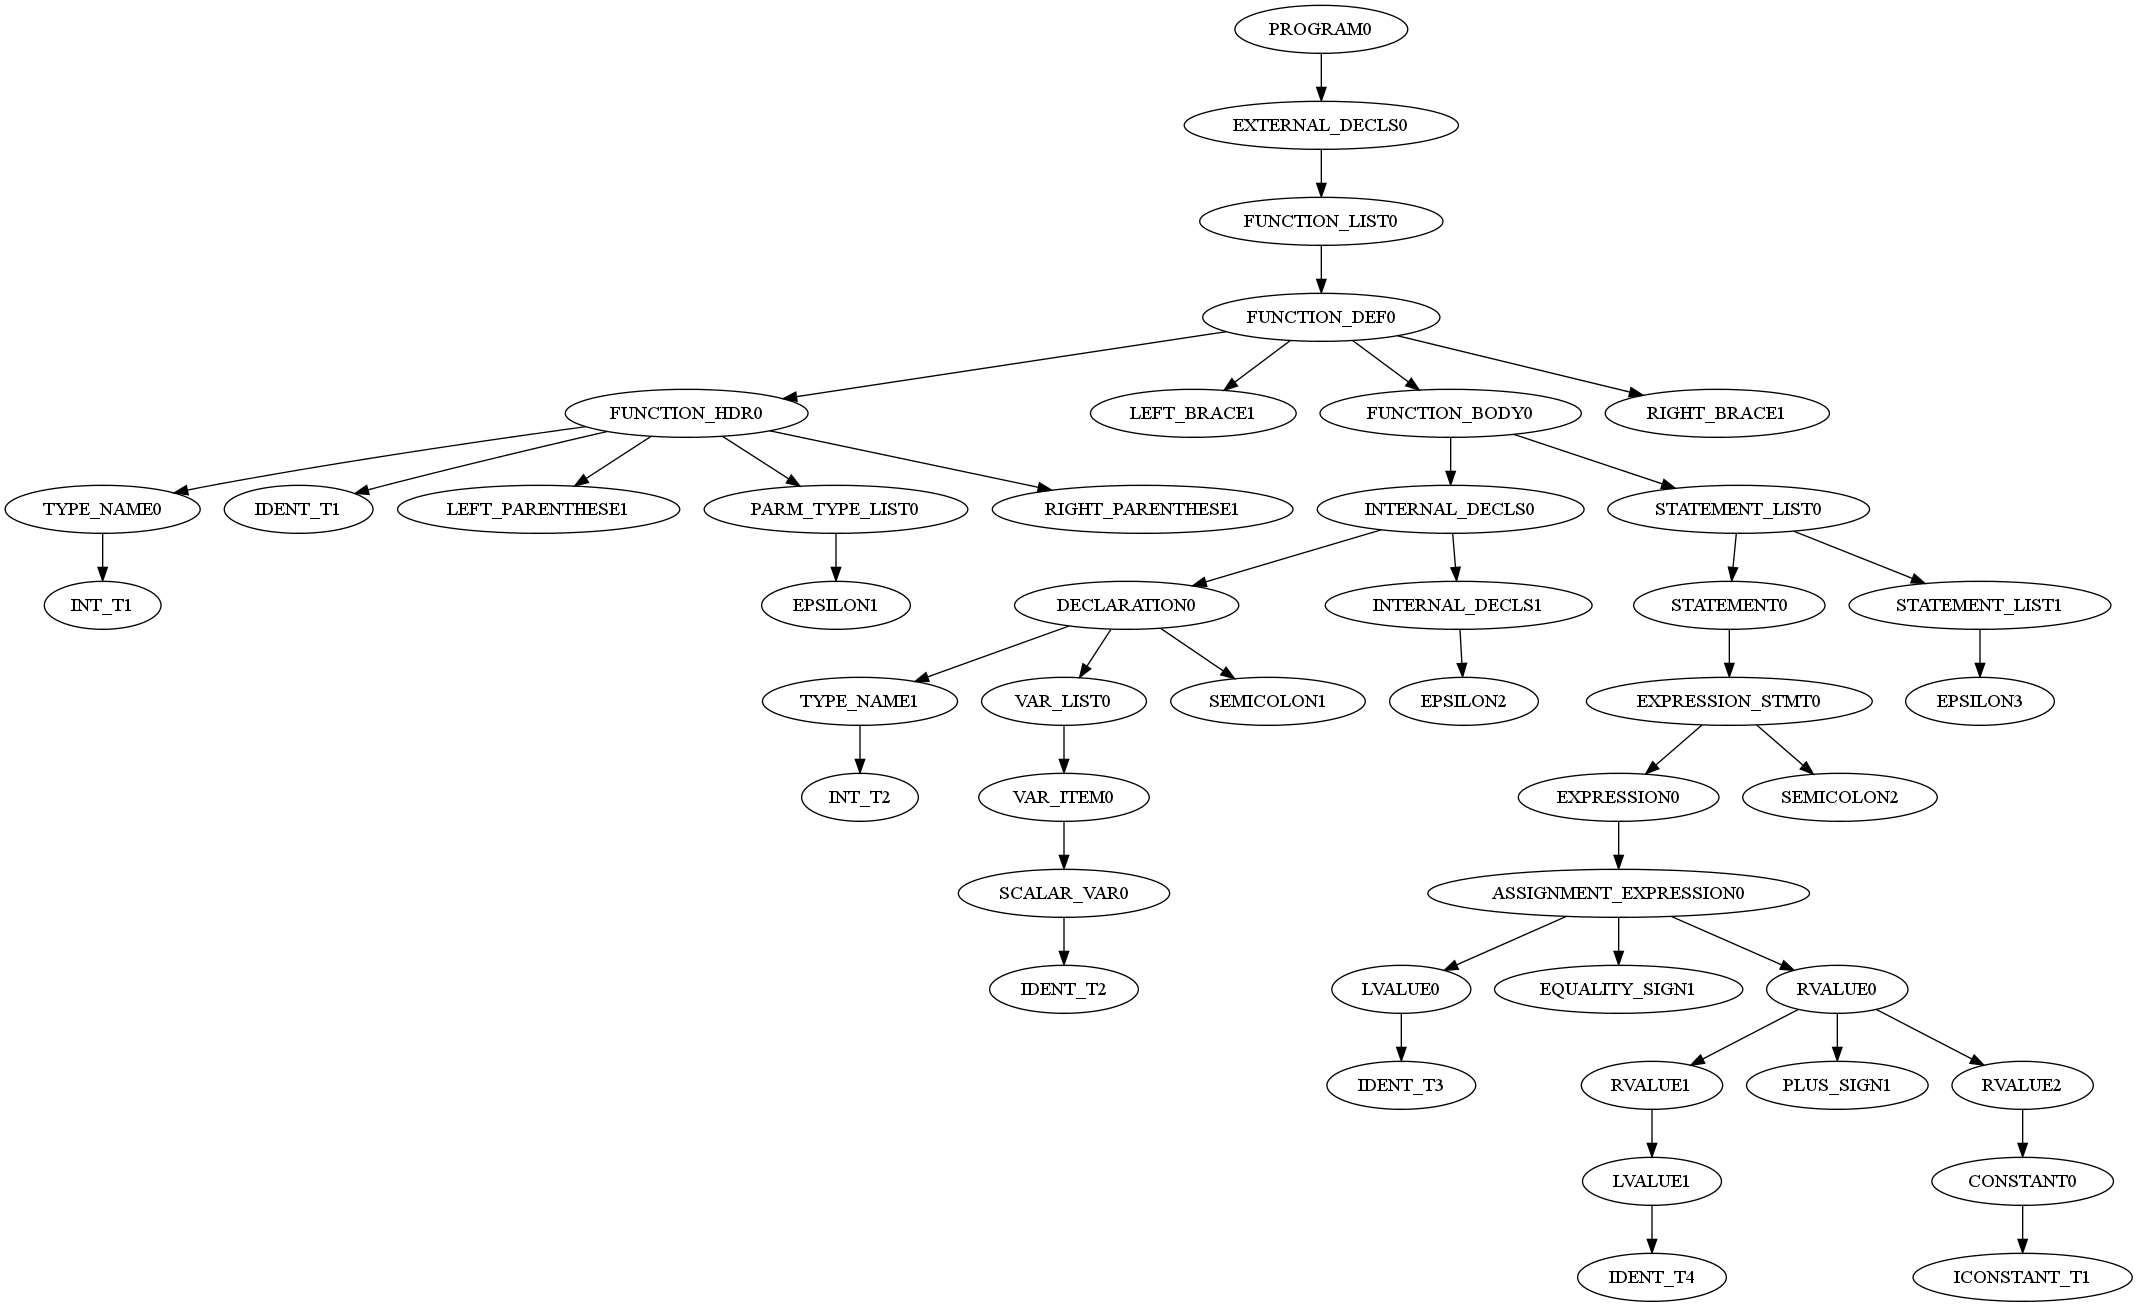
\includegraphics[scale=0.2]{grammer_tree.png}
	\captionof{figure}{AST示例}
	\label{fig:grammertree}
\end{center}
{\it \manerrarrow MiniC的验证工具中提供了两种方式查看输入源文件的语法树:\verb|dot|和ASCII ART,请参阅MiniC使用手册}\\
\subsection{AST的通用周游模板}
\label{ASTtravesal}
由于建立符号表、类型检查以及将AST变换成三元式都涉及到在AST上做深度游先周游,所以我们设计了一个通用的周游函数\verb|tree_traversal|,该函数接受两个参数:AST的根节点指针以及返回值为\verb|int|,参数为AST节点指针的函数指针的数组。由于我们将所有的节点类型都定义成了不同的整数,因此只需要为不同的周游阶段构造不同的函数指针数组,在\verb|tree_traversal|中周游到某个节点时以节点类型为数组下标定位到对这个节点进行操作的函数并调用,就能够用同一个深度游先周游函数完成不同的周游功能。\\
{\it \anchor 有关深度优先周游模板的代码,请参阅:\verb|symtbl_operation.h|}\\

\subsection{符号表}
\label{symtbl}
符号表对于一个编译程序而言是最为重要的一个部分,从它创建以后开始的每一个步骤中,“标识符”(函数名、变量名)的出现,就意味着要在符号表中找到对应的表项,提取要使用的信息。

\paragraph*{符号表的结构}
符号表的层次结构需要根据语言的特性来决定。例如在MiniC中,由于存在着全局变量、函数声明、语句块等特点,因此符号表需要组织成树状结构。

符号表的具体底层数据结构可以有很多种选择,常见的有哈希表、链表和线性表,在MiniC中,由于考虑到输入源文件的规模都较小,所以采用可扩张的线性表来实现\footnote{这种线性表在空间不足时会另外申请一块两倍的空间并拷贝自己}。在这种实现下,插入一个表项的均摊开销是$O(1)$,检索一个表项的开销是$O(n)$,$n$为表项总数目。


MiniC的符号表结构如下:
\begin{enumerate}
\item 每个作用域(函数、复合语句)一张符号表:
\begin{lstlisting}
struct symtbl_hdr
{
	symtbl_hdr* parent_tbl; //父表
	symtbl_hdr* leftChild_tbl; //最左子表
	symtbl_hdr* rightSibling_tbl;	//右兄弟子表

	//ret_type, ret_star, para_num, func are useful only for function's symtbl
	char* func_name; //函数名,若该表属于复合语句则该项为空
	int ret_type; //函数返回值基类型
	int ret_star; //函数返回值是否为指针类型
	int para_num; //该函数的参数个数
	int func_def; //该函数是否有定义
	int item_num; //符号表表项数目
	int maxSize; //全部表项占用的内存大小,字节
	symtbl_item* item; //表项列表
}
\end{lstlisting}
\item 每张符号表都有一个表项列表:
\begin{lstlisting}
struct symtbl_item
{
	int isGlobal; //是否为全局变量
	int type; //表项的基类型
	int star_num; //表项是否为指针
	int writable; //表项是否为只读类型
	char* name; //符号名 
	int size; //数组大小,非数组为0
	int func_off; //
	int offset; //在内存分配中的偏移
};

\end{lstlisting}
\end{enumerate}
注意到在一个函数的符号表中,函数的参数和它的局部变量是存放在一起的,这种将参数和局部变量视作同类的安排能够为以后的内存分配、寄存器分配等提供一些方便。



\paragraph*{在AST上生成符号表}
如前所述,AST上包含了源文件中所有的信息,因此只需要扫描AST的某些子树,提取符号名称、类型、作用域等信息,就可以生成符号表。

具体的做法是:先序深度优先周游AST,找到作用域入口(\verb|FUNCTION_DEF|和\verb|COMPOUND_STMT|)并将当前作用于压入作用域栈,然后在该作用域节点下寻找类型为\verb|EXTERNAL_DECLS|和\verb|INTERNAL_DECLS|的节点,分情况处理该节点的函数和变量的声明,将名称和类型(包括函数的返回类型,参数、参数类型)加入符号表,作用域从作用域栈顶取得。在作用域出口(周游函数返回时)弹出作用域栈顶。\\
{\it \anchor 有关符号表生成的相关代码,请参阅:\verb|gen_symtbl.h|}\\

\paragraph*{在符号表上查询符号}
由于符号表是树状组织,因此查询时要从给定的一张符号表开始,在表中查找,如果未找到符号,就在当前表的父表中查找,直到找到该符号或者在最高级的\verb|Global Scope|也没有找到返回空。
\\
{\it \anchor 有关符号表查询的代码,请参阅:\verb|symtbl_operation.h|}\\
\paragraph*{符号表生成与语义检查}
\label{declchk}
在符号表生成的过程中,实际上还要进行一项语义检查:同一作用域的多重定义问题。即在向当前符号表中添加符号时,如果该符号已经出现在了当前表中,就要报告错误,停止建立符号表。

\subsection{符号表示例}
下图展示了以下代码的符号表:
\begin{lstlisting}
int i,j;
void f(int k)
{
	int i,j;
}
int main()
{
	int i,j;
	{int k;}
}
\end{lstlisting}
\begin{center}
	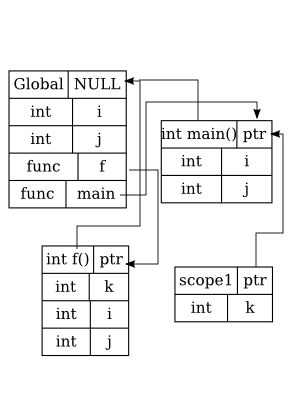
\includegraphics[scale=0.6]{symtbl.png}
	\captionof{figure}{符号表示例}
\end{center}
{\it \manerrarrow MiniC的验证工具中提供了查看源文件生成的符号表的方法:请参阅MiniC使用手册}\\
\subsection{类型检查}
\label{typeveri}
类型检查是语义检查的一部分,这一步骤的主要目的是排除所有符合语法但不符合运算规则、函数调用规则的语句。类型检查的对象是表达式语句,这包括:
\begin{itemize}
	\item 检查一元、二元运算符作用的对象;报告类型无效的运算对象
	\item 检查传入函数的实参类型和函数的参数表对应形参的类型是否兼容;报告兼容性警告或者错误
	\item 检查赋值语句两边类型是否是赋值兼容的(包括检查函数返回值);报告兼容性警告或者错误
\end{itemize}
类型检查一旦完成,表明这份源代码已经能够且必须通过后续的变换,直到生成目标代码。
\paragraph*{类型检查的规则} 下面给出了MiniC类型检查的所有规则以及应对方法。这些规则的错误/警告处理基本同\verb|gcc|的对应处理相同。

\begin{itemize}
\item 对于每个表达式,若其中有一部分类型检查返回的类型为错误类型,则直接返回错误类型。
\item 对于赋值语句,若赋值两边的表达式类型不相同,则要进行必要的转换或者报错:
	\begin{itemize}
  		\item 若赋值符号左边为指针类型,但同时又是数组类型:报错;
  		\item 若两边一边为指针,另一边为\lstinline|int|或者\lstinline|char|:警告
  		\item 若两边均为指针或者均非指针,则三元式临时变量的类型同操作数的类型;除非除非某操作数的类型为\lstinline|char|且另一操作数的类型为\lstinline|int|,此时警告,并且三元式临时变量的类型同第一个操作数类型。
  	\end{itemize}
\item 对于\hyperref[lrvalue]{左值},分以下情况:
	\begin{itemize}
		\item 若左值为一个变量,则在符号表中查找它,没找到则报错,否则正常返回一个代表该变量类型。另外,还要判断一下该变量的类型,若为\lstinline|void|类型或者声明为函数类型同样报错。
		\item 若左值为一个指针的解引用,则判断对应的被解引用的\hyperref[lrvalue]{右值}是否是一个指针类型,若是则将返回的变量类型置为普通类型。
		\item 若左值为一个数组元素,则首先检查数组头是否为指针类型,若不是则报错。其次检查数组下标对应的元素是否是一个非指针的\lstinline|int|型表达式或者一个\lstinline|char|型表达式,若不是则报错。返回对应数组元素类型即可。
	\end{itemize}
\item 对于\hyperref[lrvalue]{右值},分以下情况:
	\begin{itemize}
		\item 对应的表达式为一个单目运算符和一个操作数,则调用函数对单目运算符表达式进行类型检查。
		\item 单目运算符:
		\begin{itemize}
			\item 正号和负号:判断其操作数是否是int型变量或char型变量,若不是则报错。
			\item 对于自增运算符++和自减运算符--,若其操作数为数组变量,则报错。
		\end{itemize}

	\item 若该右值是一个无关的函数调用,则在符号表中查询该函数,若该函数没有声明为一个无参函数则报错。
	\item 若是一个双目运算符的表达式,则调用函数对双目运算符表达式进行类型检查:
	\begin{itemize}
		\item 对于关系运算符(\verb|>,<,==,<=,>=,!=|),检查两个操作数的类型,若不完全相同则警告。
		\item 对于布尔操作符(\verb+||,&&+),检查两个操作数类型,若不完全相同则警告
		\item 对于减法运算,需要报错的情况有:第一个操作数非指针,第二个操作数是指针;两个操作数均为指针,但类型不同
		\item 对于加法运算,只有当两个操作数均为指针时需要报错,其它情况进行必要的类型转换即可。
		\item 对于乘法运算,当两个操作数任何一个为指针时报错,否则进行必要的类型转换并返回即可。
	\end{itemize}
	\item 若该右值是含参数的函数调用,那么先求出所有参数类型,然后检查参数个数,若调用的参数个数与函数在符号表中的函数个数不符,则报错。否则若参数类型和函数在符号表中的参数的类型不同,则警告。
\end{itemize}
\end{itemize}
\paragraph*{在AST上做类型检查}
类似于生成符号表,类型检查同样要对AST进行深度优先周游,在发现\verb|STATMENT|类型的节点时开始按照不同的语句类型以及语句中不同的元素类型开始进行类型检查。


\section{三元式}
\label{triple}
三元式是MiniC的第二重中间表示。同MiniC源文件中复杂的语句和操作相比,三元式相对简单、只有少数指令并且更接近目标代码表示。

MiniC中,一条三元式可以表示为如下形式:
\begin{itemize}
\item A: 一般的运算指令:\verb|(i): op arg1, arg2|, \verb|arg|可以是\verb|(j)|也可以是标识符或立即数;\verb|arg2|若无效则为单元操作
\item B: 条件跳转指令:\verb|(i): if arg goto (j)|,\verb|arg|可以是\verb|(j)|也可以是标识符或立即数
\item C: 无条件跳转指令:\verb|(i): goto (j)|
\item D: 传参指令:\verb|(i): param arg|,\verb|arg|可以是\verb|(j)|也可以是标识符或立即数;出现在调用指令前
\item E: 调用指令:\verb|(i): call (j)|
\item F: 作用域指令:\verb|(i): enter|, \verb|(i): leave|用于指示作用域的变化
\item G: 布尔专用指令:\verb|(i): setrb|, \verb|(i): getrb|用于组合布尔表达式的翻译,后面会有详细叙述
\end{itemize}
\subsection{三元式的结构}
\label{triplestruct}
考虑到后续在三元式上的操作,三元式并不以上述的字符串的形式储存,以结构的形式存在一个可扩张的线性表中(类似于符号表的实现)。下面给出表项的结构:
\begin{lstlisting}
typedef struct triple
{
	enum operator op;
	union arg arg1;
	union arg arg2;
	int result_type; //运算结果的类型
	int arg1_type; //参量的类型
	int arg2_type; 
	symtbl_hdr* symtbl; //本条三元式所属范围的符号表
	struct basic_block *block; //本条三元式所属的基本块
	int arg1_uni; //“联合查询表”中第一个参数的编号
	int arg2_uni; //“联合查询表”中第二个参数的编号
	int tmp_uni; //“联合查询表”中三元式标号(临时变量)的编号
	int label; //本条三元式的标号(仅当本条三元式是跳转语句的目标时有效)
}triple;
\end{lstlisting}
有关“联合查询表”的作用,参见“机器无关优化”一节的\hyperref[jointtable]{“基础数据结构”}。
\subsection{三元式指令列表}
\label{tripleinst}
下面的表格给出了MiniC的三元式中所有的\verb|op|以及对应的功能和三元式类型(每种类型的具体解释见本节起始处的说明):
\begin{center}
\begin{minipage}{0.48\textwidth}
\begin{flushleft}
	\begin{tabular}{|l|l|l|}
	\hline
		\verb|op| & 类型 & 功能 \\
	\hline
		\verb|if| & B & 条件成立就跳转 \\
	\hline
		\verb|if_not| & B & 条件不成立就跳转 \\
	\hline
		\verb|goto| & C & 无条件跳转\\
	\hline 
		\verb|negative| & A & 取相反数\\
	\hline
		\verb|not| & A & 取布尔非\\
	\hline
		\verb|address| & A & 取地址\\
	\hline
		\verb|star| & A & 取地址处存放的数据\\
	\hline
		\verb|positive| & A & 返回操作数本身\\
	\hline
		\verb|assign| & A & 值赋给\verb|arg1|\\
	\hline
		\verb|star_assign| & A & 赋值给地址\\
	\hline 
		\verb|add| & A & 加法\\
	\hline 
		\verb|minus| & A & 减法\\
	\hline
		\verb|multiply| & A & 乘法\\
	\hline 
		\verb|char_to_int| & A & 类型转换\\
	\hline
		\verb|equal| & A & 判断相等\\
	\hline
		\verb|less| & A & 判断是否小于\\
	\hline 
		\verb|larger| & A & 判断是否大于\\
	\hline
		\verb|eqlarger| & A & 判断是否大于等于\\
	\hline
	\end{tabular} 
\end{flushleft}
\end{minipage}
\begin{minipage}{0.48\textwidth}
\begin{flushright}
\begin{tabular}{|l|l|l|}
	\hline
		\verb|op| & 类型 & 功能 \\
	\hline
		\verb|eqless| & A & 判读是否小于等于\\
	\hline 
		\verb|noteq| & A & 判读是否不等于\\
	\hline 
		\verb|or| & A & 布尔或\\
	\hline 
		\verb|and| & A & 布尔与\\
	\hline 
		\verb|setrb| & G & 将\verb|rb|置为\verb|arg|的值\\
	\hline 
		\verb|getrb| & G & 获取\verb|rb|的值\\
	\hline 
		\verb|call| & E & 调用函数\\
	\hline 
		\verb|param| & D & 传参\\
	\hline 
		\verb|enterF| & F & 进入函数\\
	\hline 
		\verb|enterS| & F & 进入复合语句\\
	\hline 
		\verb|leaveF| & F & 离开函数\\
	\hline 
		\verb|leaveS| & F & 离开复合语句\\
	\hline 
		\verb|return| & A & 返回\\
	\hline
		\verb|adds| & A & 左移两位后加\\
	\hline
		\verb|minuss| & A & 左移两位后减\\
	\hline 
		\verb|r_shift| & A & 右移两位\\
	\hline 
		\verb|c_str| & A & 表示一个字符串\\
	\hline
		\verb|Imm| & A & 表示一个大于511的立即数\\
	\hline
	\end{tabular}
\end{flushright}
\end{minipage}
	\captionof{table}{MiniC三元式\lstinline|op|定义}
\end{center}
\subsection{将AST转换为三元式}
这一工作仍然使用\hyperref[ASTtravesal]{AST的通用周游模板}进行,只是操作的对象换成了不同类型的语句(\verb|STATEMENT|)。有关一些特殊语句,例如\verb|for, while, if|的翻译,由于使用的方法同\cite{sunjiasu}的第8章对应部分相似,本文档不再赘述。下面仅介绍转化工作的最困难的部分。
\paragraph*{表达式的转换}
\label{ASTtotriple}
%TODO:表达式转换 from毛哥
\subsection{生成基本块}
\label{basicblock}
基本块,是一些机器无关的全局优化的操作对象,其定义见\cite{sunjiasu}的第9章。实际实现时,基本块的基本成员仅有几个指针,分别指向块首和块尾的三元式以及该块的前驱和后继。同时,为了方便遍历某个函数的所有基本块,我们还将所有基本块连成了一条链。注意,一个基本块的前驱可以有很多个,但后继最多只有两个。
\begin{lstlisting}
typedef struct basic_block {
	int begin; //起始三元式编号
	int end; //结束三元式编号
	int m; //本块在链表中的位置
	struct basic_block* prev; //链表中的上一块
	struct basic_block* next; //链表中的下一块
	struct basic_block* follow; //直接后继
	struct basic_block* jump; //跳转后继
	PreList* predecessor; //前驱链表
	struct func_block* fb; //所属函数
}basic_block;
\end{lstlisting}

{\it \anchor 有关基本块的完整结构的定义以及基本块的生成函数,请参阅:\verb|basic_block.h, gen_basic_block.c|}\\
\paragraph*{基本块示例}

对于以下的一个函数,它的基本块如下图所示:
\begin{lstlisting}
int main()
{
	int i;
	char p[10];
	for(i = 0 ; i < 10 ; i++){
		p[i] = 'z' - i;
	}
}
\end{lstlisting}
\begin{center}
	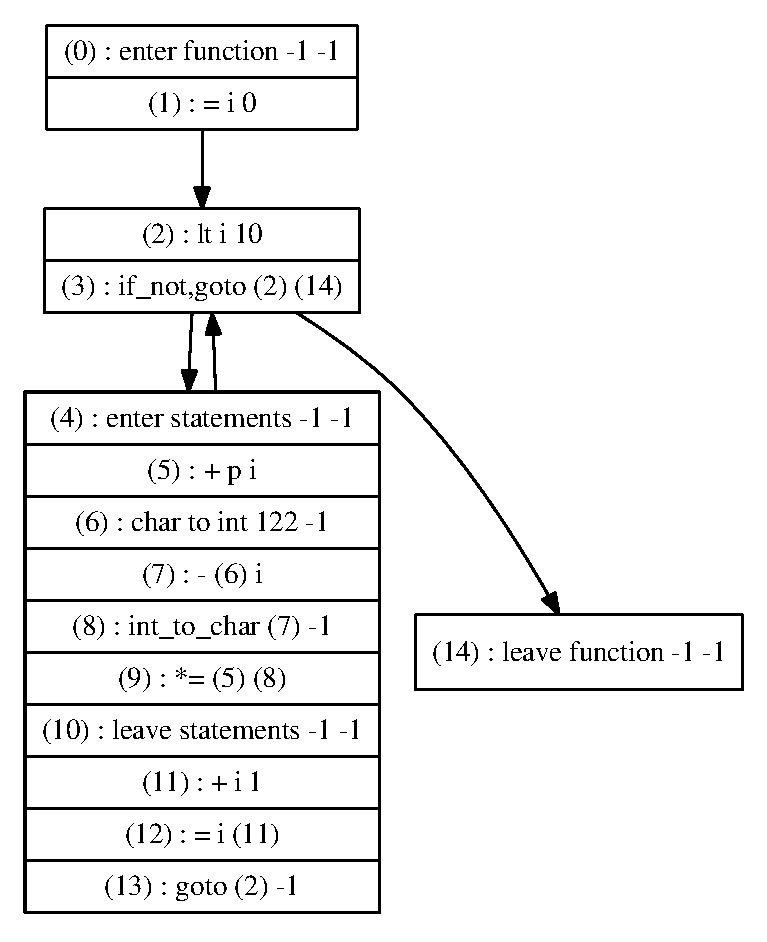
\includegraphics[scale=0.5]{basic_block}
	\captionof{figure}{基本块示例}
\end{center}
{\it \manerrarrow MiniC的验证工具中提供了生成基本块图形表示的dot文件的方法,请参阅MiniC使用手册}\\
\section{机器无关优化}
\label{indepopt}
%TODO:
MiniC在三元式表示上进行了如下优化:
\begin{itemize}
	\item 窥孔优化:常量表达式计算和面向机器的强度削减
	\item 基于数据流分析的可用表达式传播和指针分析
\end{itemize}
另外,活跃变量分析虽然不能算是优化的一部分,但由于也是基于数据流分析的迭代模型的算法,因此也在本节介绍。

\subsection{窥孔优化}
\label{peephole:intermidiate}
我们首先对三元式进行了简单的窥孔优化:
\subsubsection{常量表达式计算} 对于操作数都是常量的三元式,我们计算出该三元式的值,如果用到该三元式值的三元式又能够直接计算,那么要迭代地进行这个过程,直到结果是编译时不可计算的为止。由于目标代码生成方面的需要,这个优化不考虑对于带有常数的布尔运算。

\paragraph*{示例}
下面左图是优化前的一段三元式,右图是优化后的结果:
\begin{center}
\begin{minipage}{0.4\textwidth}
\begin{center}
	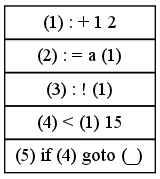
\includegraphics[scale=0.50]{before_const_expr.png}
	\label{fig:beforconstexpr}
\end{center}
\end{minipage}
\begin{minipage}{0.4\textwidth}
\begin{center}
	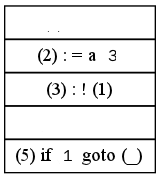
\includegraphics[scale=0.50]{after_const_expr.png}
	\label{fig:afterconstexpr}
\end{center}
\end{minipage}
\captionof{figure}{常量表达式优化示例}
\end{center}
\paragraph*{简单的强度削减} 虽然这部分是机器相关的(在Unicore32中,乘法指令需要2 CPU cycles,而移位指令仅需要1 CPU cycle),但在三元式部分做较为简单,即把乘以2的幂次的三元式都替换成左移幂次位数的三元式。在目标代码生成阶段,左移的三元式会被翻译成移位\verb|mov|,然后通过目标代码的窥孔优化将其和其它代码合并。

\subsection{数据流分析及相关优化}
\label{dataflow}
数据流分析技术都基于相似的算法框架和数据结构,只是在初值和迭代方程处不同。下面将介绍我们用于数据流分析的数据结构,并将重点介绍我们设计或改造的数据流分析算法。

数据流分析算法的范围是一个函数,因此下面的讨论的都是怎样在单个函数中进行数据流分析。

\subsubsection{基础数据结构}
\label{jointtable}
数据流分析算法具有以下特点:
\begin{itemize}
	\item 每一个“程序点”,即每个三元式之前和之后,都有不同的状态集,并且该状态集的成员可能是所有三元式(标号,也即临时变量)或所有变量
	\item 状态集成员的状态只有2种
	\item 需要多次迭代,每个基本块的输入或输出是根据其前驱的输入和输出进行交汇运算而得,交汇运算一般为集合并或集合交,因此需要能够快速进行这两种操作的集合表示。 
\end{itemize}
这些特点决定了数据流分析算法需要位向量来表示状态集,因此就会引出如何将变量或或三元式标号映射到位向量的某一位的方法;与此同时,一些算法还需要快速判断两个变量名是否代表同一个变量(因为有不同的作用域),所以我们为每一个有值的三元式建立了符号表项,并使用了一个“联合查询表”统一地保存函数中出现的所有变量和标号的符号表项指针。我们还将三元式中操作数及结果所代表的变量或标号在“联合查询表”中的位置保存了在三元式的结构中。现在,某个变量或标号在位向量中的位置就是它在“联合查询表”中的索引;比较变量相同只需判断它们在“联合查询表”中的索引是否相等。

由于是在函数范围内做数据流分析,因此我们还建立了表示一个函数的数据结构,它包含了指向该函数首、尾基本块的指针以及该函数的所有数据流分析状态信息,还包括了以后的寄存器分配信息。
\begin{lstlisting}
typedef struct func_block {
	basic_block* start; //函数入口基本块
	basic_block* over; //结束基本块
	struct func_block* prev; //函数链中上一个函数
	struct func_block* next; //函数链中下一个函数

	int code_num; //函数中三元式个数
	int bb_num; //函数中基本块个数
	symtbl_item** uni_table; //“联合查询表”
	int uni_item_num;
	int uni_table_size;
	
	map_table* mapping; //记录“联合查询表”中标号的映射信息
	int map_table_size;	
	/*活跃变量分析信息*/
	... 
	/*----------------*/
	
	/*可用表达式分析信息*/
	...
	/*------------------*/
	
	/*寄存器分配信息*/
	...
	/*------------------*/

}func_block;
\end{lstlisting}
{\it \anchor 有关\verb|func_block|的完整定义以及“联合查询表”的建立方法,请参阅:\verb|basic_block.h|, \verb|prepare_dataflow.c|}\\

活跃变量分析和可用表达式分析算法参见\cite{sunjiasu}中第9章。下面介绍两个我们改进和设计的关于数据流分析的优化算法。
\subsubsection{可用表达式传播}
这种算法只利用可用表达式信息,产生的效果类似于但劣于复写传播。

\paragraph*{目的}某些表达式在同一函数中计算了多次,需要在保证正确的情况下用第一次计算的结果代替其余计算的结果。举例如下:

在下面左图的流图中,(1)(4)(7)(9)均是相同的表达式,并且从(1)开始,a和b都没有重新定值,因此可以用(1)去替换下面出现的三元式操作数(4)(7)(9),并且删去重复计算的后三句,得到下面右图。
\begin{center}
\begin{minipage}{0.4\textwidth}
\begin{center}
	\includegraphics[scale=0.50]{before_available_expr.jpeg}
\end{center}
\end{minipage}
\begin{minipage}{0.4\textwidth}
\begin{center}
	\includegraphics[scale=0.50]{after_available_expr.jpeg}
\end{center}
\end{minipage}
\captionof{figure}{可用表达式传播示例}
\end{center}

\paragraph*{算法}
\begin{enumerate}
	\item 进行可用表达式分析
	\item 遍历三元式列表,对于一个未被修改或删除的三元式,如果它之前的程序点上有和它进行相同计算的可用表达式,那么沿着该三元式的所有非环前驱路径向上查找它所有最远的与它进行相同计算的可用表达式,如果仅找到1个,假设其标号为$i$,那么进行3,否则继续遍历三元式列表,遍历完毕则进行4。
	\item 从当前三元式向下查找所有用当前三元式标号当操作数的三元式,将该操作数替换成$i$,删除当前三元式,记录被修改的三元式,继续遍历。
	\item 如果没有三元式被删除,那么算法结束,否则进行1
\end{enumerate}
之所以进行迭代,是因为在修改三元式后,会出现新的替换机会。
\paragraph*{缺陷}
若某个三元式所计算的表达式在该点可用,但这些可用表达式没有公共的可用表达式前驱,则这种算法不能省去该三元式。例如,如果去掉上图中的(1)句,虽然插入赋值语句后再运用复写传播仍然能够将(9)省掉,但由于本算法的只进行简单的替换而不进行语句的插入,所以不能确定应当将(9)替换成(4)还是(7)。这个缺陷的更深层次的原因请见本章的\hyperref[pitfallc2]{“谬误与陷阱”}。\\

{\it \anchor 有关可用表达式传播的代码,请参阅:\verb|available_expr.c|}\\
\subsubsection{指针分析}
在面向RISC结构的处理器的C编译器实现中,为了提高运算性能,大部分的变量留在寄存器中以减少访存次数。但是指针能够直接访问变量所属的内存位置。因此,需要保证在指针操作后,某个变量在寄存器中的值和其在栈帧中的值同步,为了掌握需要将哪些变量在内存中的值更新这一信息,我们需要对三元式代码进行指针分析。
为此,我们设计了一个基于数据流分析的算法,来相对精确地得到在某一点每个指针可能指向哪些变量。
\paragraph*{算法}基于数据流分析迭代框架:
\begin{itemize}
\item 操作集合是指针-变量序对\verb|(p,v)|的集合
\item 对于每个基本块$B$,$GEN(B)$是在该块中产生的指针-变量序对(即有指针赋值或取地址操作),$KILL(B)$是在该块中注销的指针-变量序对(如果某指针指向了别的变量,就注销掉该指针以前指向的变量)
\item 迭代顺序:正向;迭代方程:$OUT(N) = GEN(N)+(IN(N)-KILL(N))$\\$IN(N)=\bigcup_{P\in predecessor(N)}OUT(P)$
\end{itemize}
\paragraph*{性能}
我们将结合一个例子来比较以下三种算法:
\begin{itemize}
	\item 假设某个指针可能指向所有变量,即遇到指针访问就同步所有的变量
	\item 扫描一遍代码,记录某个指针可能指向哪些变量,只同步可能指向的变量
	\item 基于数据流分析的指针分析
\end{itemize}
\begin{lstlisting}
int f()
{
	int a,b,c,*p,*q;
	...
	if(some_condition)
		p = &a;
	else
		p = &b;
	*p = 1;
	while(some_condition){
		q = p;
		*q = 1;
		q = &c;
		*q = 2;
	}
	...

}
\end{lstlisting}
第一种算法将在第9行、第12行和第14行将\verb|a, b, c|全部同步;第二种算法在第9行同步\verb|a, b|,在第12行和第14行同步\verb|a, b, c|;第三种算法将在第12行同步\verb|a, b|,在第12行同步\verb|a, b, c|,在第14行同步\verb|c|。

可以看出,基于数据流分析的指针分析具有更好的精确性,因此能够节省更多的内存操作的次数。\\
{\it \anchor 有关指针分析的代码,请参阅:\verb|pointer_analysis.c|}\\

\subsubsection{一些对数据流分析的改进设想}
\paragraph*{全局指针分析}
当前MiniC的指针分析算法只能得到函数内的指针可能指向的变量,但是将指针作为参数传入另一个函数后,由于得不到该指针可能指向的地址,只能在调用函数时保存所有局部变量。如果能将指针分析的范围扩大到整个源文件,那么就能够得到完整的指向信息,从而彻底地解决正确、节约地同步寄存器和内存的问题。
\paragraph*{全局活跃变量分析}
当前MiniC的活跃变量分析算法只能得到函数内的活跃变量信息。改进的可能同样来自函数调用:如果能够得到被调用的函数将占用哪些寄存器,就能够在调用前只保护这些寄存器,从而节省一些访存语句。这有赖于全局的(跨函数的)活跃变量分析。
\section{谬误与陷阱}
\label{pitfallc2}
\subsection*{中间表示设计的小缺陷将会引起许多不便}
\paragraph*{AST的修剪}
MiniC建立的AST没有经过任何修剪,从图\ref{fig:grammertree}的示例中可以看出,一些无用的语法符号(例如括号、逗号)仍然留在AST上,并且在声明和语句等子树上存在着大量的左递归子树。

在设计之初,我们忽略了这些多余的节点和复杂的左递归结构可能带来的问题。但当使用这棵AST生成了符号表并且进行了类型检查后,我们发现如果事先对AST进行一些简单的预处理,消除掉冗余的部分,替换掉复杂的结构,就能够避免使用AST时复杂的条件分支,也能够避免因为复杂的结构而造成的代码逻辑上的错误。

\paragraph*{三元式,四元式}
在设计之初,我们认为三元式和四元式在表达能力上是等价的,并且发现三元式有良好的结构使得在其上构建DAG更方便,于是MiniC采用了三元式作为第二重中间表示。

然而,三元式的特点也是它的缺点:因为标号同时也代表临时变量,因此在三元式表示中,临时变量只能赋值一次。这个缺陷影响了后面的两部分工作:
\begin{itemize}
\item 在翻译布尔表达式时,必须允许某个标志变量被赋值两次,否则布尔表达式的赋值(如\verb|a=b&&c|)将无法实现。因此我们向三元式中添加了\verb|setrb|和\verb|getrb|两条语句。虽然在目标代码生成阶段没有直接翻译这两条语句,而是转换成了效率更高,更易读的汇编代码,这种表示仍然给我们带来了不少麻烦。
\item 在进行基于三元式的优化时,由于发现了可用表达式但无法在多处插入给同一个临时变量赋值的三元式(见\cite{sunjiasu}第216页),我们只好放弃性能更为强大的可用表达式-复写传播来消除冗余中间代码,改为使用可用表达式传播的算法。
\end{itemize}
